% Copyright 2021  Ed Bueler

\documentclass[xcolor={svgnames},
               hyperref={colorlinks,citecolor=DeepPink4,linkcolor=FireBrick,urlcolor=Maroon}]
               {beamer}

\mode<presentation>{
  \usetheme{Madrid}
  \usecolortheme{seagull}
  \setbeamercovered{transparent}
  \setbeamerfont{frametitle}{size=\large}
}

\setbeamercolor*{block title}{bg=red!10}
\setbeamercolor*{block body}{bg=red!5}

\usepackage[english]{babel}
\usepackage[latin1]{inputenc}
\usepackage{times}
\usepackage[T1]{fontenc}
% Or whatever. Note that the encoding and the font should match. If T1
% does not look nice, try deleting the line with the fontenc.

\usepackage{empheq}
\usepackage{xspace}
\usepackage{verbatim,fancyvrb}

\usepackage{tikz}
\usetikzlibrary{shapes,arrows.meta,decorations.markings,decorations.pathreplacing,fadings,positioning}


% If you wish to uncover everything in a step-wise fashion, uncomment
% the following command:
%\beamerdefaultoverlayspecification{<+->}

\newcommand{\ba}{\mathbf{a}}
\newcommand{\bb}{\mathbf{b}}
\newcommand{\bc}{\mathbf{c}}
\newcommand{\bbf}{\mathbf{f}}
\newcommand{\bg}{\mathbf{g}}
\newcommand{\bn}{\mathbf{n}}
\newcommand{\bq}{\mathbf{q}}
\newcommand{\br}{\mathbf{r}}
\newcommand{\bx}{\mathbf{x}}
\newcommand{\by}{\mathbf{y}}
\newcommand{\bv}{\mathbf{v}}
\newcommand{\bu}{\mathbf{u}}
\newcommand{\bw}{\mathbf{w}}

\newcommand{\bF}{\mathbf{F}}
\newcommand{\bG}{\mathbf{G}}
\newcommand{\bQ}{\mathbf{Q}}

\newcommand{\grad}{\nabla}
\newcommand{\Div}{\nabla\cdot}
\newcommand{\minmod}{\operatorname{minmod}}

\newcommand{\CC}{\mathbb{C}}
\newcommand{\RR}{\mathbb{R}}

\newcommand{\ddt}[1]{\ensuremath{\frac{\partial #1}{\partial t}}}
\newcommand{\ddx}[1]{\ensuremath{\frac{\partial #1}{\partial x}}}
\newcommand{\Matlab}{\textsc{Matlab}\xspace}
\newcommand{\Octave}{\textsc{Octave}\xspace}
\newcommand{\eps}{\epsilon}

\newcommand{\ip}[2]{\left<#1,#2\right>}

\newcommand{\xiphalf}{{x_{i+\frac{1}{2}}}}
\newcommand{\ximhalf}{{x_{i-\frac{1}{2}}}}
\newcommand{\Fiphalf}{{F_{i+\frac{1}{2}}}}
\newcommand{\Fimhalf}{{F_{i-\frac{1}{2}}}}
\newcommand{\Fiphalfn}{{F^n_{i+\frac{1}{2}}}}
\newcommand{\Fimhalfn}{{F^n_{i-\frac{1}{2}}}}

\newcommand{\trefcolumn}[1]{\begin{bmatrix} \phantom{x} \\ #1 \\ \phantom{x} \end{bmatrix}}
\newcommand{\trefmatrixtwo}[2]{\left[\begin{array}{c|c|c} & & \\ #1 & \dots & #2 \\ & & \end{array}\right]}
\newcommand{\trefmatrixthree}[3]{\left[\begin{array}{c|c|c|c} & & & \\ #1 & #2 & \dots & #3 \\ & & & \end{array}\right]}
\newcommand{\trefmatrixgroups}[4]{\left[\begin{array}{c|c|c|c|c|c} & & & & & \\ #1 & \dots & #2 & #3 & \dots & #4 \\ & & & & & \end{array}\right]}

\newcommand{\blocktwo}[4]{\left[\begin{array}{c|c} #1 & #2 \\ \hline #3 & #4 \end{array}\right]}

\newcommand{\bqed}{{\color{blue}\qed}}
\newcommand{\ds}{\displaystyle}

\newcommand\mynum[1]{{\renewcommand{\insertenumlabel}{#1}%
      \usebeamertemplate{enumerate item} \,}}


\title{Getting started with machine learning}

\subtitle{({one little artificial neural net})}

\author{Ed Bueler}

\institute[UAF]{MATH 692 Mathematics for Machine Learning \\ University of Alaska Fairbanks}

\date[Spring 2022]{13 January 2022}

%\titlegraphic{\begin{picture}(0,0)
%    \put(0,180){\makebox(0,0)[rt]{\includegraphics[width=4cm]{figs/software.png}}}
%  \end{picture}
%}

%% this nonsense needed to start section counter at 0; see
%% https://tex.stackexchange.com/questions/170222/change-the-numbering-in-beamers-table-of-content
\makeatletter
\patchcmd{\beamer@sectionintoc}
  {\ifnum\beamer@tempcount>0}
  {\ifnum\beamer@tempcount>-1}
  {}
  {}
%\beamer@tocsectionnumber=-1
\makeatother


\begin{document}
\beamertemplatenavigationsymbolsempty

\begin{frame}
  \maketitle
\end{frame}

\begin{frame}{today's talk}

\begin{itemize}
\item \alert{my topic:} {\small how this $\downarrow$ neural network does this $\downarrow$ classification task}

\medskip
\hspace{5mm} 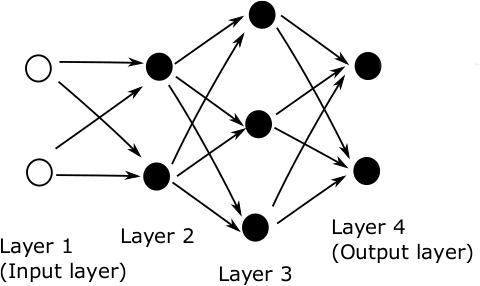
\includegraphics[height=25mm]{figs/network.png} \hfill 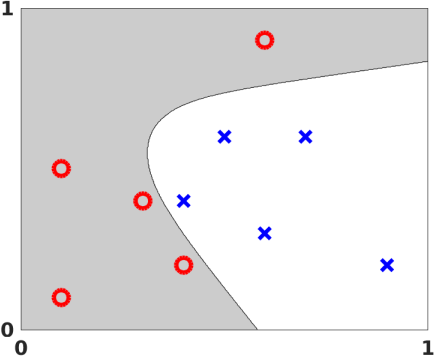
\includegraphics[height=23mm]{figs/classification} \hspace{10mm}

\medskip
\item an \alert{example} from this $\downarrow$ paper:

\medskip

HH19 \, $=$ \, 
\begin{minipage}[t]{0.75\textwidth} \footnotesize
C.~F.~Higham \& D.~J.~Higham (2019). \href{http://www.math.stonybrook.edu/~bishop/classes/math533.S21/MachineLearning/SIAMreview.pdf}{\emph{Deep learning: An introduction for applied mathematicians.}} SIAM Review, 61(4), 860-891
\end{minipage}
\end{itemize}
\end{frame}


\begin{frame}{today's talk}

\begin{itemize}
\item \alert{goal for today:} know the meanings of

\medskip
\small
\qquad \begin{tabular}{ll}
\emph{artificial neuron} \qquad & \emph{activation function} \\
\emph{weight matrix} & \emph{bias vector} \\
\emph{back-propagation} & \emph{stochastic gradient method}
\end{tabular}

\medskip
\item which standard mathematical concept(s) match these buzzwords?
\end{itemize}
\end{frame}


\begin{frame}{big caveat}

\begin{itemize}
\item I am no expert on what I am talking about here
\item many in room know more than me
\item I volunteered to give one intro talk, that's all!
\end{itemize}
\end{frame}


\begin{frame}{Outline}
  \tableofcontents[hideallsubsections]
\end{frame}


\section{seminar logistics}

\begin{frame}{\emph{participant}-driven seminar}

\begin{itemize}
\item sign-up sheet!
\item webpages:
    \begin{itemize}
    \item[$\circ$] \href{http://bueler.github.io/M692S22/index.html}{\texttt{bueler.github.io/M692S22}}
    \item[$\circ$] \href{http://bueler.github.io/M692S22/resources.htm}{\texttt{bueler.github.io/M692S22/resources.htm}}
    \end{itemize}
\item in-person or hybrid?
    \begin{itemize}
    \item[$\circ$] is this classroom adequate?
    \end{itemize}
\item what will be the topics?
    \begin{itemize}
    \item[$\circ$] are there out-of-bounds topics?
    \item[$\circ$] who is volunteering to talk?
    \end{itemize}
\end{itemize}
\end{frame}


\section{a single artificial neuron}

\begin{frame}{artificial neuron $=$ nonlinear-ized inner product}

\begin{columns}
\begin{column}{0.55\textwidth}
\begin{itemize}
\item given (column) vectors $v,w \in \RR^n$
\item inner product
    $$\ip{{\color{blue} w}}{v} = {\color{blue} w}^\top v = \sum_{j=1}^n {\color{blue} w_j} v_j$$
\item apply a nonlinear function $\sigma: \RR^1 \to \RR^1$:
\only<1>{
\begin{equation*}
{\color{red} a} = \sigma\left(\sum_{j=1}^n {\color{blue} w_j} v_j\right) \in \RR^1
\end{equation*}
}
\only<2>{
\begin{equation*}
{\color{red} a} = \sigma\left(\sum_{j=1}^n {\color{blue} w_j} v_j + {\color{ForestGreen} b}\right) \in \RR^1
\end{equation*}
}
    \begin{itemize}
    \item<2>[$\circ$] add a \alert{bias} ${\color{ForestGreen} b} \in \RR^1$
    \item[$\circ$] that's it! an \alert{artificial neuron}
    \end{itemize}
\end{itemize}
\end{column}
\begin{column}{0.45\textwidth}
\only<1>{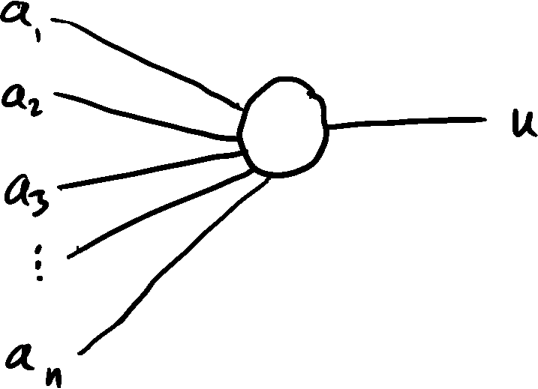
\includegraphics[width=\textwidth]{figs/single-neuron}}
\only<2>{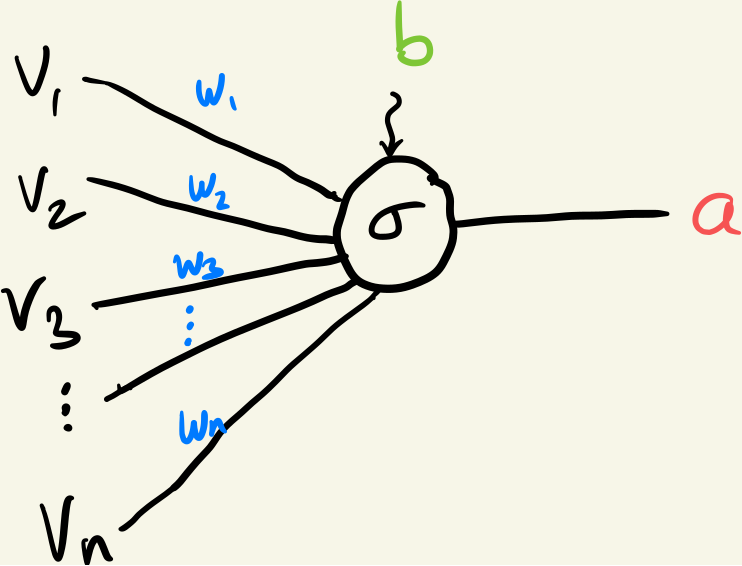
\includegraphics[width=\textwidth]{figs/b-single-neuron}}
\end{column}
\end{columns}
\end{frame}


\begin{frame}{nonlinear activation function}

\begin{center}
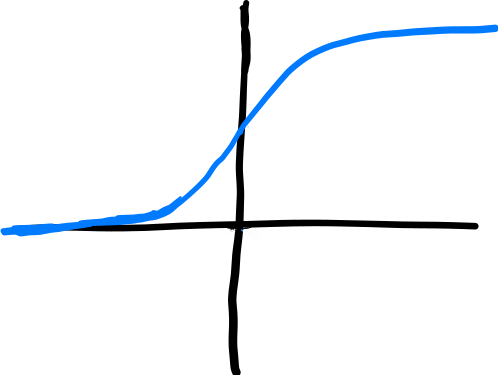
\includegraphics[height=30mm]{figs/sigmoid} \hspace{10mm} 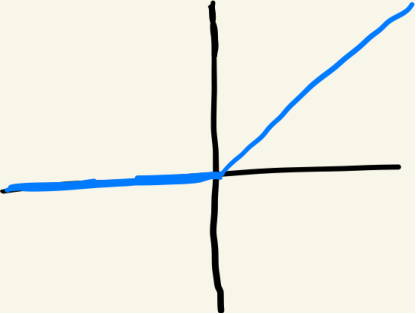
\includegraphics[height=30mm]{figs/relu}
\end{center}

\begin{itemize}
\item $\sigma$ is the \alert{activation function}
\item possibilities:
    \begin{itemize}
    \item[$\circ$] \alert{sigmoid}, e.g.\qquad $\displaystyle \sigma(z) = \frac{1}{1 + e^{-z}}$ \quad (left)
    \item[$\circ$] \alert{rectified linear unit (ReLU)},\qquad $\displaystyle \sigma(z) = \begin{cases} z, & z > 0 \\ 0, & z \le 0 \end{cases}$ \quad (right)
    \end{itemize}
\item $\sigma$ is increasing, with bounded derivative
\end{itemize}
\end{frame}


\begin{frame}{neuron roles}

\begin{columns}
\begin{column}{0.55\textwidth}
\only<1>{
\begin{itemize}
\item $v$ is input
\item $\sigma$ is fixed
\item $a$ is the \alert{activation} of the neuron
\item $w,b$ are parameters
\end{itemize}
}
\only<2>{
\begin{itemize}
\item parameters are determined by \alert{training}
\item a \alert{trained neuron} is one with fixed parameters
\item function $a:\RR^n \to \RR^1$:
    $$a = \sigma(v)$$

    \begin{itemize}
    \item[$\circ$] similar cost to inner product
    \item[$\circ$] backward stable
    \end{itemize}
\item one might write when training:
    $$a = \sigma(v;w,b)$$
\end{itemize}
}
\end{column}
\begin{column}{0.45\textwidth}
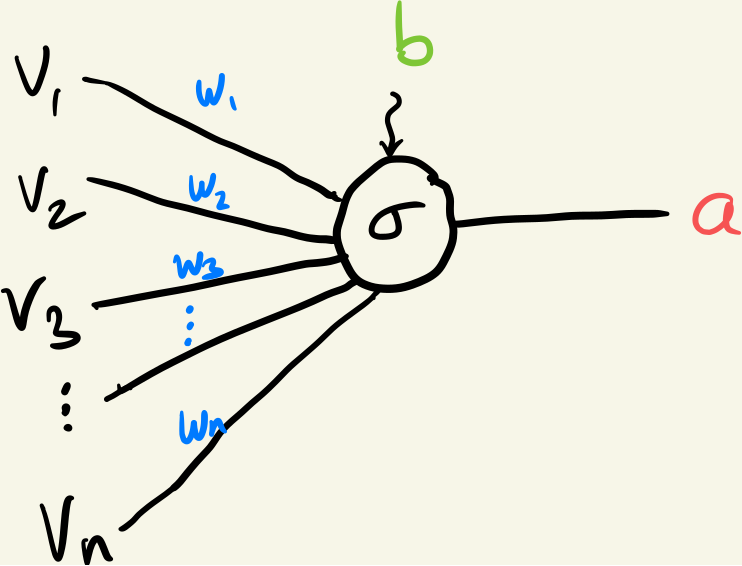
\includegraphics[width=\textwidth]{figs/b-single-neuron}
\end{column}
\end{columns}
\end{frame}


\section{forward through a neural net}

\begin{frame}{network notation}

\begin{center}
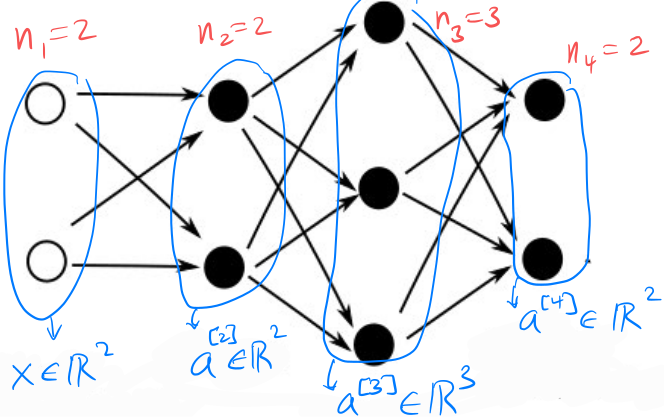
\includegraphics[height=40mm]{figs/state-notation}
\end{center}

\begin{itemize}
\item notation from HH19
\item ${\color{red} n_\ell}$ is number of neurons in layer $\ell=1,\dots,L$
    \begin{itemize}
    \item[$\circ$] $\ell=1$ is \alert{input} layer (for passing-in values $x = {\color{blue} a^{[1]}} \in \RR^{{\color{red} n_1}}$)
    \item[$\circ$] $\ell=L$ is \alert{output} layer
    \end{itemize}
\item activations from layer $\ell$ are a vector ${\color{blue} a^{[\ell]}} \in \RR^{{\color{red} n_\ell}}$
    \begin{itemize}
    \item[$\circ$] ${\color{blue} a_j^{[\ell]}}$ is activation of neuron $j$ in layer $\ell$
    \item[$\circ$] we label a neuron by its activation: ``neuron ${\color{blue} a_j^{[\ell]}}$''
    \end{itemize}
\end{itemize}
\end{frame}


\begin{frame}{network notation}

\begin{center}
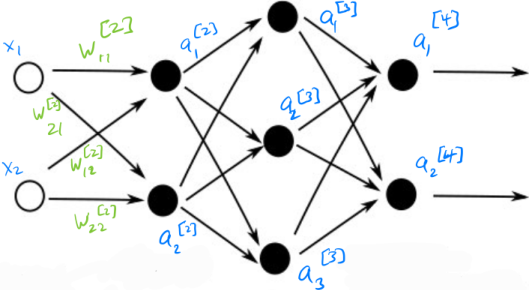
\includegraphics[height=40mm]{figs/weight-notation}
\end{center}

\only<1>{
\begin{itemize}
\item assumption made \emph{here}: the network is \alert{feed-forward}, and edges only connect consecutive layers
    \begin{itemize}
    \item[$\circ$] in language of graph theory: connected, directed acyclic graph (DAG) which is equal to its own transitive reduction \dots I think
    \item[$\circ$] versus \alert{recurrent}
    \end{itemize}
\end{itemize}
}
\only<2>{
\begin{itemize}
\item weight ${ \color{ForestGreen} w_{jk}^{[\ell]} }$ on the edge from neuron ${\color{blue} a_k^{[\ell-1]}}$ to neuron ${\color{blue} a_j^{[\ell]}}$
\item thus
    $${\color{blue} a_j^{[\ell]}} = \sigma\left(\sum_{k=1}^{n_{\ell-1}} {\color{ForestGreen} w_{jk}^{[\ell]}} {\color{blue} a_k^{[\ell-1]}} + b_j\right)$$
\item which suggests matrix multiplication!
\end{itemize}
}
\end{frame}


\begin{frame}{vector/matrix network notation}

\begin{center}
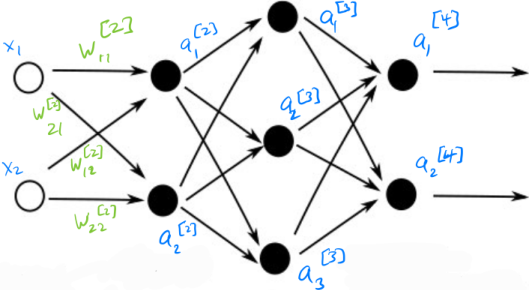
\includegraphics[height=40mm]{figs/weight-notation}
\end{center}

\begin{itemize}
\item one row vector $w^\top$ of weights for each neuron, thus many neurons deserve a matrix:
    $${\color{ForestGreen} W^{[\ell]}} = \left(\text{weights into layer $\ell$}\right) = \begin{bmatrix} {\color{ForestGreen} w_{jk}^{[\ell]}} \end{bmatrix} \quad \text{is } n_{\ell}\times n_{\ell-1}$$
\item assume $\sigma$ applied entrywise, thus
    $${\color{blue} a^{[\ell]}} = \sigma\left({\color{ForestGreen} W^{[\ell]}} {\color{blue} a^{[\ell-1]}} + b^{[\ell]}\right)$$
with $b^{[\ell]} \in \RR^{n_{\ell}}$
\end{itemize}
\end{frame}


\begin{frame}{forward pass = nonlinear-ized matrix multiplication}

\begin{center}
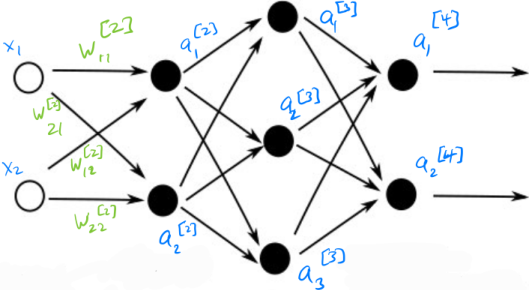
\includegraphics[height=25mm]{figs/weight-notation}
\end{center}

\begin{itemize}
\item for this small $L=4$ network:
\begin{align*}
y = a^{[4]} &= \sigma\left(W^{[4]} a^{[3]} + b^{[4]}\right) = \dots \\
            &= \sigma\left(W^{[4]} \sigma\left(W^{[3]} \sigma\left(W^{[2]} a^{[1]} + b^{[2]}\right) + b^{[3]}\right) + b^{[4]}\right) \\
            &= \sigma\left(W^{[4]} \sigma\left(W^{[3]} \sigma\left(W^{[2]} x + b^{[2]}\right) + b^{[3]}\right) + b^{[4]}\right)
\end{align*}
\item if $\sigma(z)=z$ and $b^{[\ell]}=0$ then $y = W^{[4]} W^{[3]} W^{[2]} x$
\item feed-forward network = nonlinear \& affine matrix multiplication
\end{itemize}
\end{frame}


\begin{frame}{computation work model}

\begin{itemize}
\item x
\item beamer
\end{itemize}
\end{frame}


\section{backward through a neural net}

\begin{frame}{fixme}

\begin{itemize}
\item latex
\item beamer
\end{itemize}
\end{frame}


\section{training is just optimization}

\begin{frame}{fixme}

\begin{itemize}
\item latex
\item beamer
\end{itemize}
\end{frame}


\section{running the codes yourself}

\begin{frame}{\emph{Matlab online} instructions: HH19 codes}

\begin{itemize}
\item as a UAF person you have access to Matlab online if you want it

\begin{center}
\href{https://matlab.mathworks.com/}{\texttt{matlab.mathworks.com}}
\end{center}

    \begin{itemize}
    \item[$\circ$] I also use Octave
    \end{itemize}
\item 
\item beamer
\end{itemize}
\end{frame}


\begin{frame}{\emph{Matlab online} instructions: my versions of HH19 codes}

\begin{itemize}
\item FIXME
\item beamer
\end{itemize}
\end{frame}


\section{things that bother me}

\begin{frame}{fixme}

\begin{itemize}
\item latex
\item beamer
\end{itemize}
\end{frame}

\end{document}
